The architectural design for the sound vest has three major layers: Music Player, Music Filter, and Music Amplification/Speakers. Starting with the first layer, Music Player, the layers directly interact with the layer below it. 

\begin{figure}[h!]
	\centering
 	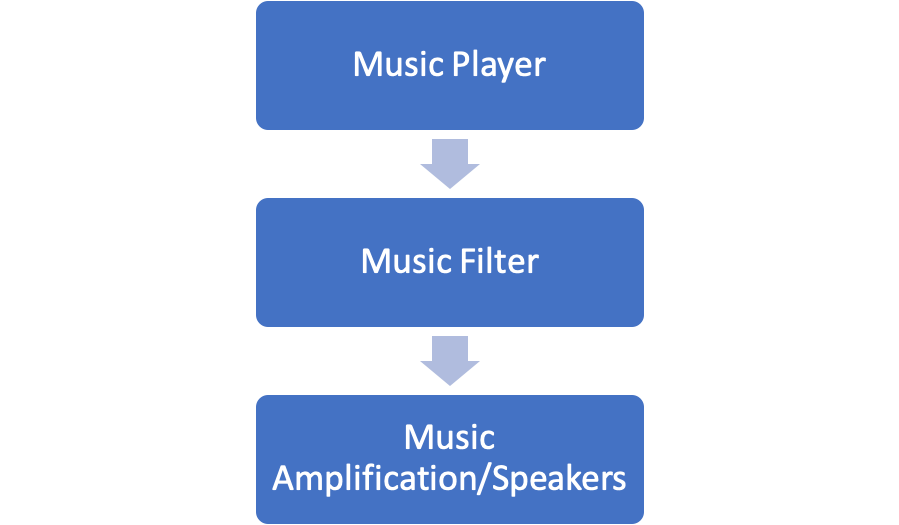
\includegraphics[width=0.60\textwidth]{images/layers}
 \caption{A simple architectural layer diagram}
\end{figure}

\subsection{Music Player Description}
The first Layer needs to be able to play music on a website. The raspberry Pi will be used as the computer to log in to the website and play the music. The music will be output from the Raspberry Pi's audio jack into the next layer. 

\subsection{Music Filter Description}
The second layer takes in the music as the input and modifies it before playing it on the speakers. First, the music passes through a pre-amplifier which will allow the music to be heard through the speakers. Next, the amplified music will be filtered through a circuit that will separate and send the different frequency ranges to different areas on the vest.

\subsection{Audio Amplification/Speakers Description}
 The final layer adjusts the music to the users liking. The user will have the option to adjust the volume/intensity of the music. Once the music is adjusted, the music will pass through shakers that will vibrate to the music being played.